%
%
%
%

\documentclass{article}
         
\usepackage{graphicx,xcolor}
\usepackage[load-headings]{exsheets}
%\usepackage{bbding, skull}
\usepackage[frenchb]{babel}
\usepackage{amsmath,amssymb,amsthm,bm}
\usepackage{enumitem}
\usepackage{lmodern,microtype}
\usepackage[a4paper,left=4cm,right=4cm]{geometry}
\usepackage{tikz}
\usepackage{hyperref}



\newtheorem{theorem}{Theorem}
\newtheorem{lemma}[theorem]{Lemma}
\newtheorem{proposition}[theorem]{Proposition}
\newtheorem{corollary}[theorem]{Corollary}
\newtheorem{conjecture}[theorem]{Conjecture}


\usetikzlibrary{arrows,decorations,calc}
\usetikzlibrary{decorations.pathmorphing,patterns,decorations.pathreplacing,decorations.markings}

\usepgflibrary{arrows}

\tikzset{
  % style to apply some styles to each segment of a path
  on each segment/.style={
    decorate,
    decoration={
      show path construction,
      moveto code={},
      lineto code={
        \path [#1]
        (\tikzinputsegmentfirst) -- (\tikzinputsegmentlast);
      },
      curveto code={
        \path [#1] (\tikzinputsegmentfirst)
        .. controls
        (\tikzinputsegmentsupporta) and (\tikzinputsegmentsupportb)
        ..
        (\tikzinputsegmentlast);
      },
      closepath code={
        \path [#1]
        (\tikzinputsegmentfirst) -- (\tikzinputsegmentlast);
      },
    },
  },
  % style to add an arrow in the middle of a path
  mid arrow/.style={postaction={decorate,decoration={
        markings,
        mark=at position .55 with {\arrow[#1]{stealth}}
      }}},
}



\renewcommand{\i}{\mathrm{i}}
\newcommand{\diff}{\text{d}}



\begin{document}
\noindent
{\textsc{Universit\'e catholique de Louvain}} \hfill \'Ecole de Physique\\
Facult\'e des Sciences \hfill 21 November 2024\\
\hrule

\bigskip

\begin{center}
  \textbf{LPHYS2114 Non-linear Dynamics}\\
  \textbf{S\'erie 8 -- Superstable fixed points, basins of attraction and conjugation} 
\end{center}

%\bigskip
\SetupExSheets{headings=runin-fixed-nr}

%\begin{question}
%  \textbf{Orbite de p\'eriode $\bm 2$.}
%  Soit l'it\'eration $x_{n+1}=f(x_n),\, n\geqslant 0$ avec $f(x) = x^2+c$.
%  \begin{enumerate}[label=(\alph*)]
%    \item Pour quelles valeurs de $c$ existe-il une orbite p\'eriodique de p\'eriode $2$ attractive/stable?
%    \item Une orbite p\'eriodique est appel\'ee superstable lorsque le produit des d\'eriv\'ees le long l'orbite vaut z\'ero. Pour quelles valeurs de $c$ l'orbite de p\'eriode $2$ est-elle superstable?
%  \end{enumerate}
%\end{question}

\begin{question}
  \textbf{Newton-Raphson Method.} Show that the fixed points of the map of the Newton-Rhapson method are superstable.
\end{question}


\begin{question}
  \textbf{Basins of attraction.} Given a function $f$ on $\mathbb R$. The \textit{basin of attraction}, of a fixed point $p$ of the map, is defined by the collection of points $x$ which converge towards $p$. The following theorem can help with finding a basin of attraction of $p$:
  \begin{theorem}
    Given a continuous $f$ on $\mathbb R$ and $a<b<c$.
    \begin{enumerate}[label=(\roman*)]
      \item If $f(b)=b$ and $x<f(x)<b$ for all $x\in [a,b[$ then $\lim_{n\to \infty}f^n(a) = b$.
      \item If $f(b)=b$ and $b<f(x)<x$ for all $x\in ]b,c]$ then $\lim_{n\to \infty}f^n(c) = b$.
    \end{enumerate}
  \end{theorem}
  \noindent The first part of this exercise consists in demonstrating this theorem. The second part uses the theorem for finding the basins of attraction of attracting fixed points.
  \subsubsection*{Demonstrating the theorem}
  \noindent We will only demonstrate section \textit{(i)}. (The demonstration of part \textit{(ii)} follows in a similar manner.)
  \begin{enumerate}[label=(\alph*)]
    \item Given $x_0=a$ and $x_{n+1} = f(x_n),\,n\geqslant 0$. Show that $(x_n)_{n=0}^\infty$ is a strictly increasing series. Show that it converges.
    \item Given that $p=\lim_{n\to \infty} x_n$. Justify that $a\leqslant p \leqslant b$. Deduce that $p=b$.
  \end{enumerate}
  \subsubsection*{Applications}
   \begin{enumerate}[label=(\alph*),resume]
    \item Given $f(x) = \frac{4}{\pi}\arctan x$. Show that $f$ has fixed points $p=0,\pm 1$. Show that $p=0$ is a source and $p=\pm 1$ are the attractors. Show that the basin of attraction of $p=\pm 1$ are $\{x\in \mathbb R:\pm x > 0\}$.
    \item Given $f(x) = a x(1-x)$. Show that for $1 < a < 2$ the basin of attraction of the fixed point $p=1-1/a$ is the open interval $]0,1[$.
  \end{enumerate}
\end{question}
  
\begin{question}
  \textbf{Conjugation.} In this exercise we consider the maps that can be linked by conjugation.
  
  \subsubsection*{Example}
  \begin{enumerate}[label=(\alph*)]
    \item Show that the logistic map $x_{n+1}=ax_n(1-x_n)$ can be transformed into the map $y_{n+1} = y_n^2 + c$ by a linear change of variables $y_n = \alpha x_n+\beta$ with $\alpha,\beta$ which are to be determined.
 
    \item Show that we can write the relation between the maps in the form
    \begin{equation}
      C\circ f = g \circ C
      \label{eqn:Conjugation}
    \end{equation}
    where $C(x) = \alpha x + \beta$, $g(x) = x^2+c$ et $f(x) = a x (1-x)$.
    \end{enumerate}
    
    \subsubsection*{Properties of corresponding maps}
  \noindent More generally, two functions $f,g$ linked by a homeomorphism $C$ according to \eqref{eqn:Conjugation} are called (topological) conjugates. The properties of the dynamics of the maps can be linked. Here we consider the relations between their periodic points.
  
  \begin{enumerate}[label=(\alph*),resume]
    \item Show that $f^k$ and $g^k$ are conjugates by $C$ for all integers $k\geqslant 1$. 
    \item Show that $p$ is a $k$-periodic point of $f$ iff $C(p)$ is a $k$-periodic point of $g$.
    \item Show that if $f,g,C$ are differentiable and if $C'(p)\neq 0$ then 
    \begin{equation}
      (g^k)'(C(p)) = (f^k)'(p).
    \end{equation}
  
  \end{enumerate}
  \subsubsection*{Application: Logistic map with $\bm{a=4}$}
  \noindent
  In this part we consider the logistic map $g(x) = ax(1-x)$ with $a=4$ and \textit{The tent map}
  \begin{equation}
     f(x) =
     \begin{cases}
       2x,& 0 \leqslant x \leqslant 1/2,\\
       2(1-x) & 1/2 \leqslant x \leqslant 1,
     \end{cases}
  \end{equation}
  on the interval $[0,1]$. The graphs of the functions $f,g$ are shown in  Figure \ref{fig:Tent}.
 \begin{enumerate}[label=(\alph*),resume]
    \item Show that $f$ and $g$ are conjugates by $C(x) = \frac{1}{2}(1-\cos \pi x)$.
    \item Show that the periodic orbits of $g$ are repulsive. \textit{Hint:} Start with $k=1$ and $k=2$, and then generalise.
 \end{enumerate}
 
 \begin{figure}[h]
 \centering
 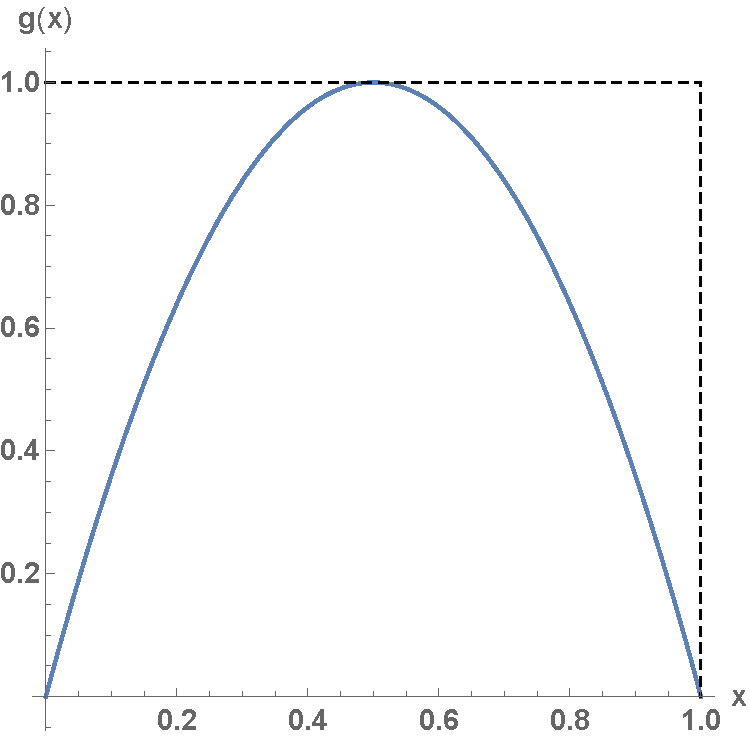
\includegraphics[width=.45\textwidth]{Logistic} 
 \hspace{.07\textwidth}
 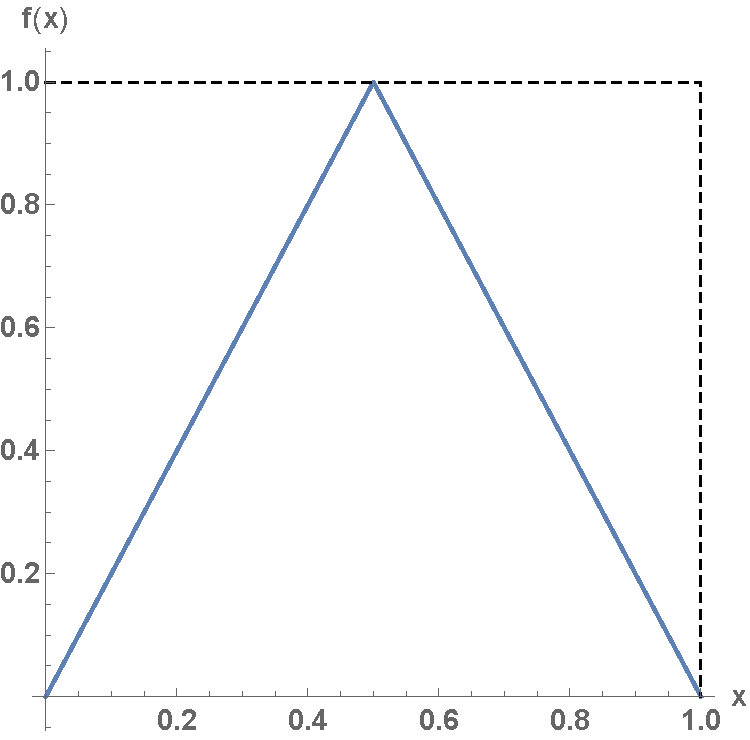
\includegraphics[width=.45\textwidth]{Tent}

 \caption{Logistic map $a=4$ (left) and the tent map (right).}
 \label{fig:Tent}
 \end{figure}
   
\end{question}




 
\end{document}

